\documentclass[9pt]{beamer}
\usefonttheme[onlymath]{serif}
\usepackage[sfdefault]{roboto}
\usepackage[utf8]{inputenc}
\usepackage[T1]{fontenc}
\usepackage{styles/fluxmacros} 	% Define where theme files are located. 
\usefolder{styles}
\usetheme[style=gray]{flux} % Available styles: asphalt, blue, red, green, gray 



\usepackage{graphicx}
\usepackage{amsmath}
\usepackage{amssymb}
\usepackage{amsfonts}
\usepackage{hyperref}

\title{Computerpraktikum Maschinelles Lernen}
\subtitle{Thema 4 - Klassifikationsverfahren}
\author{Pascal Bauer, Raphael Millon, Florian Haas}
\institute{Sommersemester 2020}
\date{\today}
\titlegraphic{assets/Empty.png}

\begin{document}

\titlepage 

\begin{frame}
 \frametitle{Table of contents}
 \tableofcontents
\end{frame}

\section{Theorie}
\begin{frame}{Theorie}{Theorie}

\end{frame}

\section{Showcase}
\begin{frame}{Showcase}{Showcase}

\end{frame}

\begin{frame}{Showcase}{Klassifikationsergebnisse für brute\_sort}
Die Klassifikationsergebnisse für \textit{brute\_sort} mit $k_\text{max} = 200, l = 5$:
\begin{center}
\begin{tabular}{|c|c|c|c|}
\hline
\textbf{Datensatz:}& \textbf{Laufzeit (in Sekunden):} & \textbf{$\text{k}^*$:} & \textbf{Fehlerrate:}\\

\hline

australian & 0.20 & 126 & 0.1346\\

\hline

bananas-1-2d  &11.4 &36 &0.2083\\

\hline

bananas-1-4d  &21.92 &48 &0.2088\\

\hline

bananas-2-2d  &11.08 &75 &0.2122\\

\hline

bananas-2-4d  &21.30 &32 &0.2213\\

\hline

bananas-5-2d  &10.96 &89 &0.2555\\

\hline

bananas-5-4d  &22.07 &175 &0.2542\\

\hline

 cod-rna.5000 &18.61 &8 &0.0693\\

\hline

 ijcnn1 &1150.36 &1 &0.0299\\

\hline

ijcnn1.10000  &41.12 &2 &0.0247\\

\hline

ijcnn1.5000  &10.01 &2 &0.0173\\

\hline

svmguide1  &5.10 &20 &0.0343\\

\hline



toy-2d  &11.35 &100 &0.2153\\

\hline

 toy-3d &18.95 &62 &0.2288\\

\hline

toy-4d  &21.89 &39 &0.2240\\

\hline

toy-10d  &45.28 &112 &0.2140\\

\hline


\end{tabular}
\end{center}
\end{frame}

\begin{frame}{Showcase}{Testen mit anderen Daten}
\textbf{Frage:} Was passiert, wenn wir als Testdaten andere Datensätze verwenden?
\begin{center}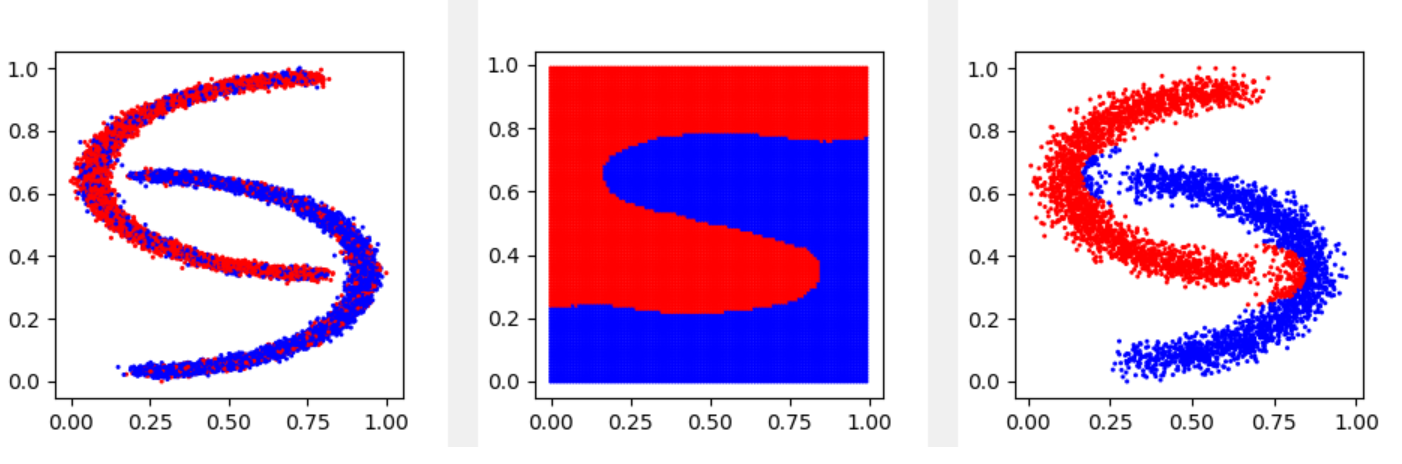
\includegraphics[scale=0.25]{assets/changed_test_data.png}\end{center}
\begin{center}\begin{tiny}(Von links nach rechts: Trainingsdaten (bananas-1-2d), Gitter, Ergebnis (mit Testdaten bananas-2-2d))\end{tiny}\end{center}
\begin{center}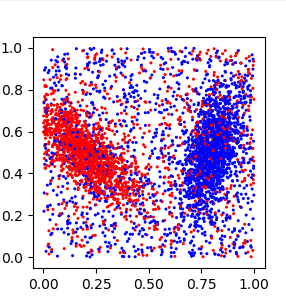
\includegraphics[scale=0.33]{assets/toy-2d.png}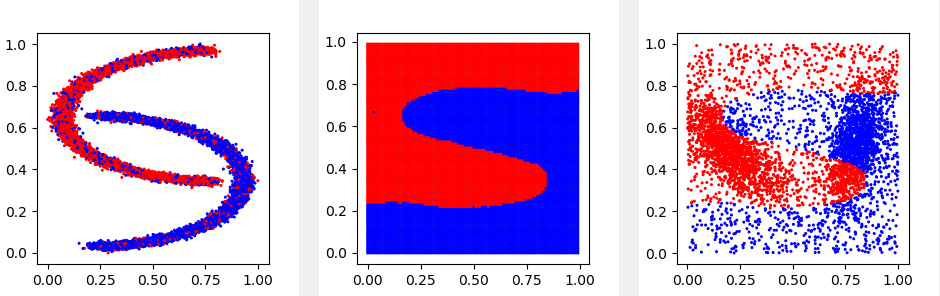
\includegraphics[scale=0.33]{assets/changed_test_data2.png}\end{center}
\begin{center}\begin{tiny}(Von links nach rechts: Testdaten (toy-2d), Trainingsdaten (bananas-1-2d), Gitter, Ergebnis)\end{tiny}\end{center}
\end{frame}

\section{Ausgesuchte Codebeispiele}
\begin{frame}{Codebeispiele}{Struktur und Module}
Code ist Open-Source auf Github: \url{https://github.com/raphaelMi/computerpraktikum-maschinelles-lernen}\\[0.4em]
Unser Programm ist in folgende Module aufgeteilt:
\begin{itemize}
\item{\textbf{main.py}: Hauptmodul mit wesentlichen Algorithmen}
\item{\textbf{dataset.py}: Datensatz-Import/-Export}
\item{\textbf{gui.py}: Grafische Oberfläche}
\item{\textbf{kd\_tree.py}: Hilfsmodul für k-d-Search}
\item{\textbf{visual.py}: Plotting der Datensätze}
\end{itemize}

Verwendete Bibliotheken:
\begin{itemize}
\item{\textbf{numpy}: Effizientes (vektorisiertes) Rechnen}
\item{\textbf{matplotlib}: Generieren der Plots}
\item{\textbf{tkinter}: Grafische Benutzeroberflächen}
\item{\textbf{scikit-learn}: Ein dritter Algorithmus zum Vergleich}
\end{itemize}
\end{frame}
\begin{frame}{Codebeispiele}{Klassifikation}
Die \textbf{classify}-Funktion ist das "Herz" unseres Programmes:
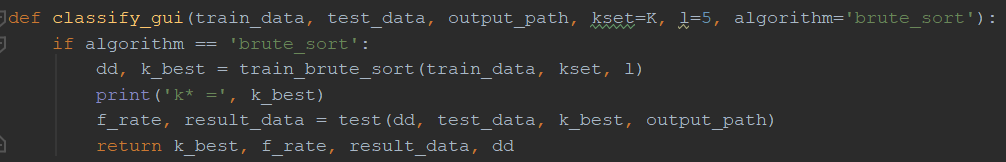
\includegraphics[scale=0.633]{assets/classify_brute.png}\\[0.4em]
Parameter:
\begin{itemize}
\item{\textbf{train\_data}: Trainingsdaten}
\item{\textbf{train\_data}: Testdaten}
\item{\textbf{output\_path}: Ausgabedatei der Ergebnisdaten}
\item{\textbf{kset}: Menge der k}
\item{\textbf{l}: Partitionsanzahl}
\item{\textbf{algorithm}: Suchalgorithmus für Nachbarn}
\end{itemize}
Ablauf:
\begin{enumerate}[1.]
\item{Training mit gegebenen Trainingsdaten und Sortieralgorithmus}
\item{Klassifikation und der Testdaten und Darstellung der Resultate}
\end{enumerate}
\end{frame}

\begin{frame}{Codebeispiele}{Training}
Nun wird $k^*$ ermittelt:
\begin{center}
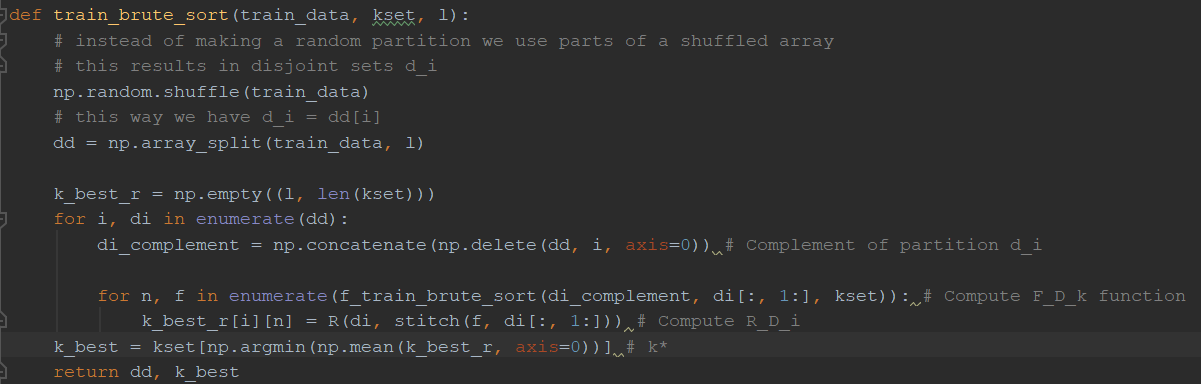
\includegraphics[scale=0.5]{assets/train_brute.png}
\end{center}
Ablauf:
\begin{enumerate}[1.]
\item{Partitionierung des Datensatzes gemäß $l$}
\item{Klassifikation und der Testdaten und Darstellung der Resultate}
\item{Berechnung des $f_{D, k}(x)$ mittels brute\_search}
\item{Berechnung der $\mathcal{R}_{D_i}$}
\item{Ermitteln des $k^*$ über Minimierung des Mittelwertes}
\end{enumerate}
\end{frame}

\begin{frame}{Codebeispiele}{Training - Teilfunktionen}
Die Berechnung der $f_{D, k}(x)$ läuft wie folgt:
\begin{center}
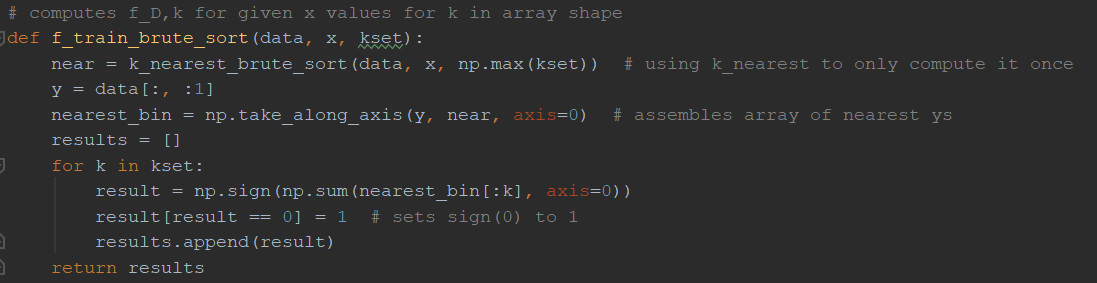
\includegraphics[scale=0.6]{assets/train_brute_sort.png}
\end{center}
Ablauf:
\begin{enumerate}[1.]
\item{Ermitteln der k-nächsten Nachbarn mittels brute\_sort}
\item{Berechnung der $f_{D, k}(x)$ nach Vorschrift für alle $k$}
\end{enumerate}
Wir berechnen die k-nearest einmal für das größte k - \textbf{k\_nearest\_brute\_sort} gibt die k-nearest nach Distanz sortiert zurück, sodass die übrigen k-nearest daraus abgeleitet werden können.
\end{frame}

\begin{frame}{Codebeispiele}{Training - Brute Sort}
Algorithmus zur Ermittlung der k-nächsten Nachbarn.
\begin{center}
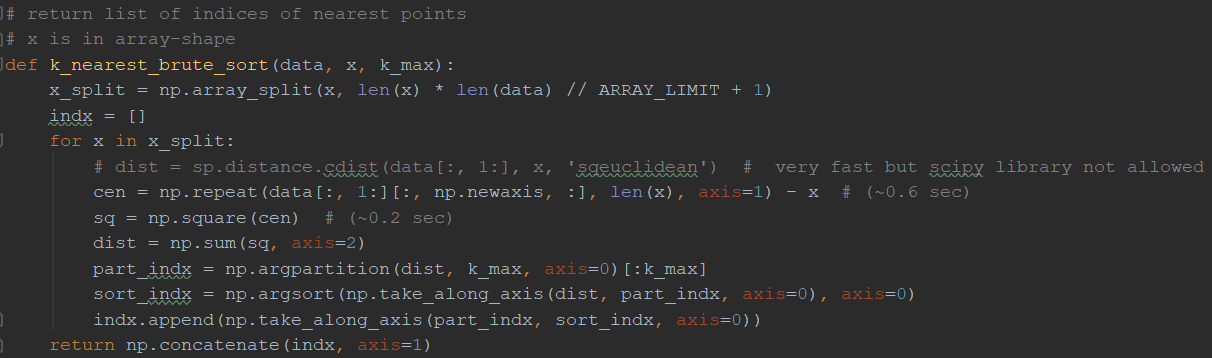
\includegraphics[scale=0.52]{assets/train_brute_sort_impl.png}
\end{center}
\end{frame}
\end{document}